% #############################################################################
% This is Chapter 6
% !TEX root = main.tex
% #############################################################################
% Change the Name of the Chapter i the following line
\fancychapter{Personalization \& Customization}
\clearpage
% The following line allows to ref this chapter
\label{chap:chap006}

\noindent
{\it Chapter~\ref{chap:chap006} was published in a conference rated A* in 2023:}

\vspace{0.5mm}

\begin{itemize}
\item {\bf Francisco Maria Calisto}, Jo\~{a}o Fernandes, Margarida Morais, Carlos Santiago, Jo\~{a}o M. Abrantes, Nuno J. Nunes, and Jacinto C. Nascimento. 2023. Assertiveness-based Agent Communication for a Personalized Medicine on Medical Imaging Diagnosis. Proceedings of the 2023 CHI Conference on Human Factors in Computing Systems (CHI '23), April 23--28, 2023, Hamburg, Germany. Association for Computing Machinery, New York, NY, USA, Article 13, 1–20. DOI: \href{https://doi.org/10.1145/3544548.3580682}{doi.org/10.1145/3544548.3580682}
\end{itemize}

Until now, this thesis explored the factors influencing the acceptance and adoption of \ac{AI} systems (Chapter~\ref{chap:chap004}), where we found enough evidence for the needs of different user groups.
Then, we delved into designing interventions (Chapter~\ref{chap:chap005}) to enhance the acceptance and integration of \ac{AI} systems in healthcare settings.
In this chapter, our focus shifts to understanding how \ac{AI} systems should communicate to address the specific needs and characteristics of different user groups~\cite{10.1145/3544548.3580682}, particularly considering the professional experience of the clinician.

\section{Motivation}
\label{sec:chap006001}

\ac{AI} systems, driven by \ac{DL} techniques, hold promise for various healthcare applications~\cite{CALISTO2022102285, Hannun2019, Ruamviboonsuk2019}.
However, these systems often fail to capture the variability among clinicians, such as interns, juniors, middles, and seniors~\cite{Uddin2019}.
Integrating technological advancements in the clinical workflow, such as \ac{AI} systems, can potentially advance personalized and precision medicine~\cite{HO2020497, Wetzstein2020}.
Consequently, understanding how \ac{AI} systems should communicate (Figure~\ref{fig:fig097}), considering the professional experience of the clinician (Section~\ref{sec:chap004006001} of Chapter~\ref{chap:chap004}), becomes a crucial design question~\cite{pacheco2019alignment}.

%%%%%%%%%%%%%%%%%%%%%%%%%%%%%%%%%%%%%%%%%%%%%%%%%%%
\begin{figure}[htpb]

\includegraphics[width=\textwidth]{fig097}
\caption[]{A sample of ``Non-Assertive'' ({\it e.g.}, suggesting ``it looks like'') {\it vs.} ``Assertive'' ({\it e.g.}, imposing ``must'') communications.}
\label{fig:fig097}
\end{figure}
%%%%%%%%%%%%%%%%%%%%%%%%%%%%%%%%%%%%%%%%%%%%%%%%%%%

This study explores the application of the BreastScreening-AI framework in two conditions: conventional and assertiveness-based agents~\cite{pacheco2019alignment, 10.1145/3311350.3347162}.
By serving as a second reader, the intelligent agents aim to enhance diagnostic performance, reduce \acp{FP} and \acp{FN} (Over-Diagnosis {\it vs} Under-Diagnosis), and improve the efficiency and efficacy of the clinical workflow~\cite{CALISTO2022102285, 10.1145/3311350.3347162}.
While much research has focused on improving the accuracy of \ac{AI} algorithms, there is a necessity to address the adoption (Chapter~\ref{chap:chap004}) and usability (Chapter~\ref{chap:chap005}) concerns of interactive assistance techniques.
This study sheds light on clinicians' needs, practices, and attitudes toward \ac{AI}-powered assistance, emphasizing the importance of personalized communication and explanations to foster trust and acceptance of \ac{AI} systems~\cite{10.1145/3491102.3502104, CALISTO2021102607}.

Through a within-subject study involving 52 clinicians, our research examines the interaction between conventional and assertiveness-based agents in diagnosing a dataset of 289 patients~\cite{PELAU2021106855}.
The assertiveness-based agent utilizes different communication tones while providing human-interpretable clinical arguments to explain the \ac{AI} algorithms' diagnostic outputs~\cite{10.1145/3544548.3580682}.
This integration of \ac{DL} methods into communication theories allows us to explore the impact of assertiveness-based \ac{AI} mediation on clinicians with varying expertise levels (Section~\ref{sec:app005001} of Appendix~\ref{chap:app005}), specifically addressing critical medical decision-making scenarios~\cite{Aldoj2020}.
The findings from our study contribute to computational interaction approaches (Section~\ref{sec:app005017}), providing valuable insights into the design of interactive systems underpinned by computational principles for the \ac{HCI} community, particularly in high-stakes domains.

\vspace{1.50mm}

\noindent
The main contributions of this work are summarized as follows (detailed in Section~\ref{sec:app005002} of Appendix~\ref{chap:app005}):

\vspace{0.05mm}

\begin{enumerate}
\item Our novel approach customizes \ac{AI}-assisted medical reasoning, demonstrating the positive impact of assertiveness-based communication on clinical workflows.
\item We show that explaining \ac{AI} outputs improve medical efficiency, but its impact depends on the communication tone of the clinical arguments.
\item Our results show that assertiveness-based agents increase the utility of clinical information and user trust in \ac{AI} recommendations without compromising diagnostic performance.
\item We offer design considerations to adapt communication in \ac{AI}-assisted reasoning based on medical expertise levels, paving the way for future implementations of personalized intelligent agents.
\end{enumerate}

\vspace{0.50mm}

The following sections outline related works on the issues of guiding the \ac{HAII} topic, assisting clinical decision-making, going through some examples of \acp{CDSSe} present in the literature~\cite{NAISEH2023102941, 10.1145/3531146.3533193}, and ending on the effects of \ac{AI} communication.
We then introduce the design of our {\it Assertiveness-based BreastScreening-AI} assistant, followed by our research questions, hypotheses, and methods.
Last, we report our quantitative and qualitative findings, concluding with a discussion of design considerations.

\section{Related Work}
\label{sec:chap006002}

Medical imaging systems enable end-users to diagnose various modalities, including \ac{MG}, \ac{US}, and \ac{MRI}, through seamless data retrieval~\cite{10.1145/3544548.3580682}.
Integrating these modalities presents opportunities for quantitative imaging and diagnoses, necessitating specialized data handling, post-processing, and visualization methods~\cite{Igarashi:2016:IVS:2984511.2984537}.
In the clinical domain, medical imaging tools aid experts in making better decisions, such as identifying cancer prognostics from multi-modal data~\cite{10.1145/3399715.3399744}.
This chapter focuses on understanding different aspects and expectations of a \ac{CDSSe} integrated into the radiology workflow (Section~\ref{sec:app005003}), highlighting the enhancement of medical imaging diagnosis through assertiveness-based interaction.

In the context of \ac{HAII}, intelligent agents must go beyond providing results alone and consider user behaviors during decision-making~\cite{10.1145/3313831.3376807}.
In Section~\ref{sec:app005003001} of Appendix~\ref{chap:app005}, we delve deeper into this \ac{HAII} literature.
Additionally, we explore the interdisciplinary topic of \ac{XAI}, which intersects cognitive psychology, learnability, and context awareness within the field of \ac{HCI}~\cite{doi:10.1073/pnas.1618211113}.
Learnability, an essential aspect of usability, encompasses various aspects such as hints, guidance, and visualizations when designing \ac{XAI} systems\cite{10.1145/3173574.3174156}.
Furthermore, explainable context awareness simplifies context representation, providing users with information about the obtained data and system actions~\cite{10.1145/3313831.3376545}.

\ac{HAII} incorporates human feedback in model training to create better \ac{ML} models~\cite{10.1145/3290605.3300233, 10.1145/3132272.3134111, Kocielnik:2019:YAI:3290605.3300641, aha2017ai}, where we bring the topic focusing on personalized and customized \ac{AI} suggestions tailored to varying levels of medical expertise (Section~\ref{sec:app005003001}).
Researchers emphasize the importance of explaining \ac{AI} systems' reasoning to enhance \ac{HAII}, particularly in medical domains, where the interpretability of \ac{AI} predictions is crucial~\cite{10.1145/3411764.3445717, Rudin2022, Kawamleh2022}.
However, these approaches often fail to account for cognitive bias in decision-making, which varies among individuals with different levels of expertise and knowledge~\cite{https://doi.org/10.1111/nuf.12430, Seidel2021}.
Our work addresses these gaps by studying assertiveness-based communication in \ac{AI} systems, considering expertise levels to reduce cognitive bias.

The integration of \ac{AI} systems into clinical decision-making is a complex endeavor (Section~\ref{sec:app005003002} of Appendix~\ref{chap:app005}), as it presents challenges and unintended consequences~\cite{miller2019intrinsically}.
Critical decisions related to patient safety, clinician fatigue, and increased medical errors need to be carefully addressed~\cite{10.1093/jamia/ocab291, 10.1117/12.2613082, doi:10.1148/radiol.212631}.
Clinicians often find \ac{AI} systems challenging to use due to limited technical skills and a lack of customization to their behavioral aspects~\cite{CALISTO2022102922}.
Additionally, the understanding and communication of \ac{AI} outcomes to clinicians are hindered by poorly designed interfaces.
These interfaces often fail to consider the differences in clinician characteristics during decision-making, such as the varying reasoning approaches between novice and expert clinicians~\cite{Edgar2022}.

The lack of large-scale deployment of \ac{AI} systems in healthcare further complicates the understanding of how these systems are perceived and used in real-world settings~\cite{10.1145/3411764.3445432, SU202328, ZAPPATORE20231}.
While approaches such as \ac{iML}~\cite{10.1145/3544548.3580682}, \ac{HITL}~\cite{10.1145/3397481.3450668}, human-\ac{AI} symbiosis~\cite{JARRAHI2018577}, and human-\acs{AI} collaboration~\cite{10.1145/3411764.3445432} have been proposed in \ac{HCI}, they primarily focus on improving prediction accuracy, model efficiency, and interpretability without adequately considering the burden on healthcare professionals~\cite{10.1145/3555157, 10.1145/3397481.3450668}.
Existing studies on the perception and usage of \ac{AI} systems for clinical decision-making often overlook potential differences in behavioral reasoning.
Additionally, some approaches solely prioritize accurate algorithmic suggestions without accounting for the clinician's professional medical experience~\cite{10.1145/3491102.3502104}.
A more detailed literature review concerning these topics is further described in Section~\ref{sec:app005003002} of Appendix~\ref{chap:app005}.
Our research bridges the gaps between \ac{HCI} and \ac{AI} approaches, focusing on personalized and customized algorithmic suggestions based on varying levels of medical expertise.
These approaches empower clinicians, improves decision-making, and enhances patient care outcomes.

\acp{CDSSe} have greatly benefited from \ac{DL} algorithms~\cite{esteva2019guide} in various applications (Section~\ref{sec:app005003003} of Appendix~\ref{chap:app005}).
\ac{DL} systems have demonstrated their ability to detect patterns, make predictions, and assist clinicians in high-stakes decision-making processes~\cite{10.1145/3555157}, such as skin cancer diagnosis~\cite{Esteva2017}, cardiac \ac{MRI} segmentation~\cite{medley2019segmenting}, and breast cancer detection~\cite{MAICAS2019101562}.
These models have shown exceptional performance in identifying meaningful patterns within medical data, sometimes surpassing human capabilities~\cite{10.1145/3544548.3580682}.
However, there is a need to adapt the communication tone of \acp{CDSSe} for personalized and customized medicine~\cite{MAICAS2019101562, CALISTO2022102285}, considering the unique behavioral characteristics and expertise levels of clinicians.
While \ac{DL}-based \acp{CDSSe} have shown promising results~\cite{McKinney2020, Rajpurkar2022}, there are challenges in translating them from research and development environments to real clinical settings.

Utility to clinicians and logistical hurdles are common obstacles in clinical adoption~\cite{CALISTO2022102922}, and some systems have not effectively reduced clinician workload~\cite{KOHLI2018535} or improved diagnostic accuracy~\cite{KOHLI2018535}.
\ac{HCI} research in clinical environments has explored the evaluation of interactive \ac{DL} systems from a human-centered perspective~\cite{10.1145/3311957.3359433, 10.1145/3359206, 10.1145/3538882.3542790}.
Studies have investigated techniques to enhance diagnostic utility and user trust in \ac{DL} predictions, as well as identified important information for clinicians when integrating \ac{AI} assistants into routine practice~\cite{10.1145/3290605.3300234, 10.1145/3359206}.
However, these studies (Section~\ref{sec:app005003003}) have yet to consider the heterogeneous behavioral nature of decision-making among clinicians.

Trust plays a critical role in communication (Section~\ref{sec:app005003004} of Appendix~\ref{chap:app005}), especially in clinical environments where life-altering decisions are made~\cite{CALISTO2022102922}.
Positive motivational attribution and reducing ambiguity through trust~\cite{HOHENSTEIN2020106190} are key factors in successful collaboration between humans and \ac{AI}~\cite{10.1145/3479587, 10.1145/3334480.3375147, 10.1145/3334480.3382842}.
The impact of assertiveness-based \ac{AI} mediation on novice and expert clinicians is still not well understood~\cite{Lundberg2020}.
Understanding the effects of \ac{AI} communication is vital to avoid unforeseen clinical consequences.
Trust directly influences clinicians' perception of \ac{AI} outcomes and their attitudes, satisfaction, and performance evaluations~\cite{10.1145/3491102.3502104}.
Attribution theory and external cues shape clinicians' interpretation of information~\cite{10.1145/3544548.3580682}.
Our work introduces assertive communication theories into a deep learning system and clinical scenario, offering a novel approach to address these dynamics.

\section{Assertiveness-based System}
\label{sec:chap006003}

In this chapter, we explore how human-\ac{AI} interactions are affected by the ability of an \ac{AI} agent to not only incorporate granular patient information from the \ac{AI} outputs but also exploring how to adapt the communication tone ({\it i.e.}, more assertive or suggestive) depending on the medical experience ({\it i.e.}, novice or expert) of the clinician.
Specifically, we compare the \ac{AI} outputs (Figure~\ref{fig:fig096} and Figure~\ref{fig:fig112}) that explain to clinicians some clinical arguments with more granular information about the patient regarding the lesion details, to a conventional agent that only provides numeric estimates ({\it e.g.}, \ac{BI-RADS} and accuracy) of the classification.
Further details are described in Section~\ref{sec:app005004} of Appendix~\ref{chap:app005}.

%%%%%%%%%%%%%%%%%%%%%%%%%%%%%%%%%%%%%%%%%%%%%%%%%%%
\begin{figure}[htpb]
\centering
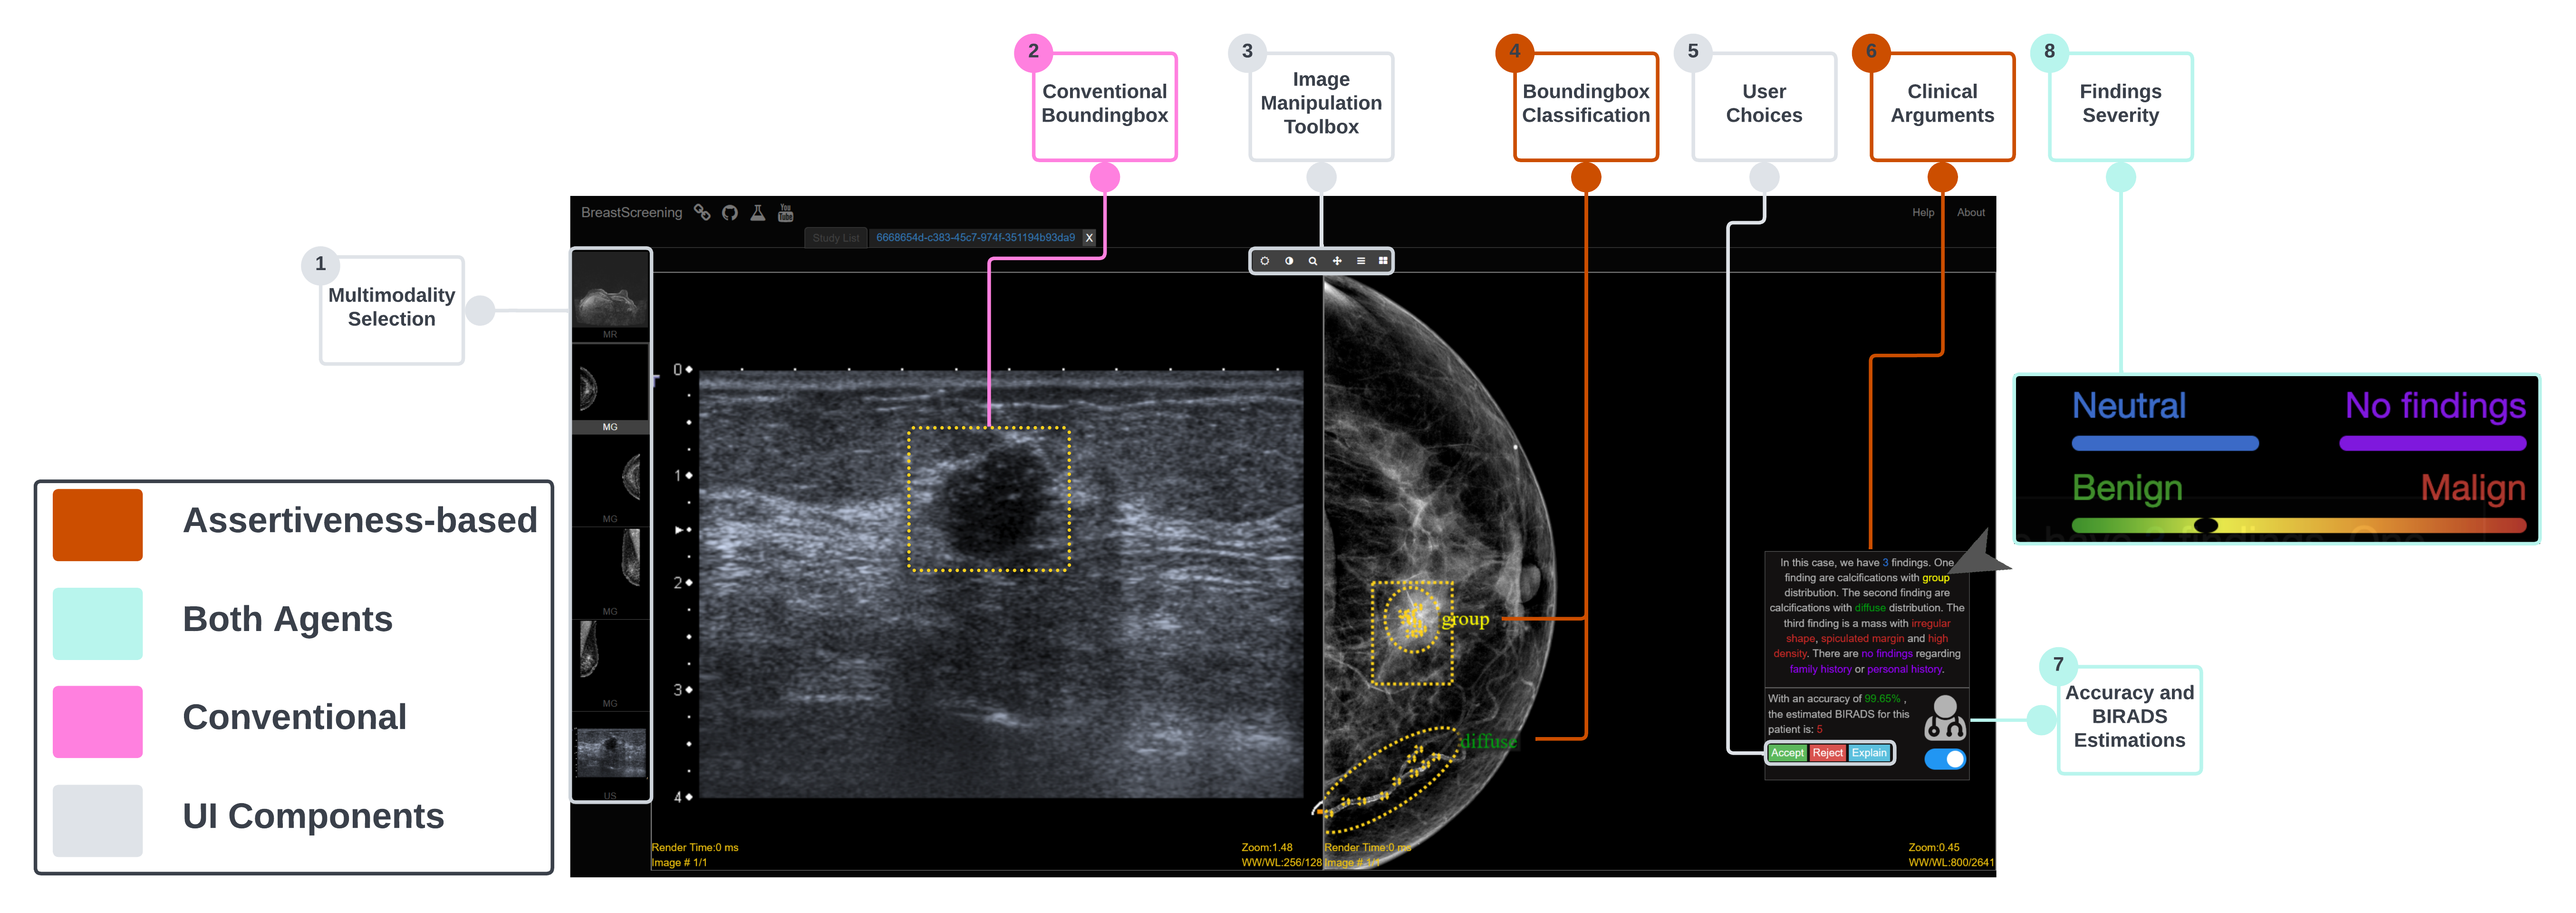
\includegraphics[width=1.000\textwidth]{fig096}
\caption[]{Interface for conventional and assertiveness-based AI agents for medical imaging analysis. Attributes are associated with numbers in each condition. AI agent provides severity information when hovering over variables. Colors range from benign (green) to malign (red). Number of findings displayed in neutral color (blue). Clinicians use purple color for family and personal history variables.}
\label{fig:fig096}
\end{figure}
%%%%%%%%%%%%%%%%%%%%%%%%%%%%%%%%%%%%%%%%%%%%%%%%%%%

Our assertiveness-based agent uses recommendations for classifying and segmenting:
(1) the number of detected findings;
(2) the patient severity of each breast and per medical imaging modality;
(3) a visual scale representing the benign or malign estimates;
(4) providing visualization of the sensitivity and specificity outcomes of the models; and
(5) with clinical arguments of the patient, such as pathological co-variables.
To compare the assertiveness-based agent to the conventional agent \textcolor{revised}{(Figure~\ref{fig:fig098}, Section~\ref{sec:app005004} of Chapter~\ref{chap:app005})}, we inform participants that the recommendations are generated by our \ac{AI} models so that they can also provide some feedback concerning the model performance.

Figure~\ref{fig:fig096} illustrates how the two \ac{AI} agents were integrated into an existing medical workflow for the classification of medical imaging data in support of breast cancer diagnosis.
Both agents are recommending classification and segmentation based on the DenseNet model~\cite{8721151} for \ac{MG} and \ac{US}, as well as based on the ResNet model~\cite{10.1145/3544548.3580682} for \ac{MRI}.
The two \ac{AI} agents provided the severity classification (Section~\ref{sec:app005009} of Appendix~\ref{chap:app005}) of the patient via \ac{BI-RADS}~\cite{SPAK2017179}, the accuracy of the model for that classification, and the segmentation of the lesion to explain the regions that derived from that classification.

\section{Research Questions \& Hypotheses}
\label{sec:chap006004}

The final purpose of our research is twofold.
Through assertiveness-based agents, we first aim to understand how personalized and customized communication could affect medical assessments in terms of the efficiency and efficacy of the clinical workflow.
Secondly, we aim to understand how clinicians perceive assertiveness-based agents differently.
Thus, our work addresses two primary research questions concerning the impact of assertiveness-based agents on efficiency and efficacy (RQ6.1), as well as the perception (RQ6.2) of clinicians.
We provide a more detailed view in Section~\ref{sec:app005005} of Chapter~\ref{chap:app005}.

\noindent
Specifically, we consider the following research questions and related hypotheses:

\vspace{0.5mm}

% New RQs
%%%%%%%%%%%%%%%%%%%%%%%%%%%%%%%%%%%%%%%%%%%%%%%%%%%
\begin{itemize}
\item {\bf RQ6.1.} How does an assertiveness-based agent affect medical assessments?
\begin{itemize}
\item {\bf H6.1.1.} Efficiency of clinicians in terms of time performance per each diagnosed patient will be higher with an assertiveness-based agent.
\item {\bf H6.1.2.} Classification accuracy of clinicians will not suffer with an assertiveness-based agent.
\item {\bf H6.1.3.} Through assertiveness-based communication, accuracy differences between novice and expert clinicians will depend on the tone of the personalized explanations.
\end{itemize}
\item {\bf RQ6.2.} How is an assertiveness-based agent perceived by clinicians?
\begin{itemize}
\item {\bf H6.2.1.} Clinicians will have a preference for an assertiveness-based agent.
\item {\bf H6.2.2.} Clinicians will consider an assertiveness-based agent more trustworthy.
\item {\bf H6.2.3.} Personalized highlights and explanations will not increase clinicians' workload nor decrease usability.
\item {\bf H6.2.4.} Novice and expert clinicians will perceive reliability and capability differently, depending on the levels of assertiveness.
\end{itemize}
\end{itemize}
%%%%%%%%%%%%%%%%%%%%%%%%%%%%%%%%%%%%%%%%%%%%%%%%%%%

In real-world clinical settings, clinicians' time is a limited and expensive resource that should be reallocated efficiently.
We take the position that while clinicians should make their clinical assessments with care, \ac{AI} agents can help with diagnosis efficiency.
Our assertiveness-based agent is designed to summarize the recommendations and to provide clinical arguments explaining the underlying classification and segmentation of the \ac{AI} models.

\section{Methods}
\label{sec:chap006005}

\textcolor{revised}{This study explores personalized and customized communication techniques in intelligent agents, particularly emphasizing the assertiveness and tone used in interactions between clinicians and intelligent agents.
More details are presented in Section~\ref{sec:app005006} in Appendix~\ref{chap:app005} for an in-depth understanding of our methodology.
From March to June 2022, we engaged with clinicians through 52 semi-structured interviews and user tests.
These were further enriched by contributions from experts in \ac{ML} and \ac{HCI}.
Our diverse group of participants, primarily healthcare professionals, participated in this study under the ethical guidelines approved by their respective institutions.
Focus groups were essential, fostering interactive discussions between clinicians and researchers.
These sessions deepened our understanding of clinician preferences and perceptions about \ac{AI} communication styles, significantly influencing the design and implementation of the intelligent agents.}

\textcolor{revised}{To rigorously assess the impact of communication styles adopted by intelligent agents on clinical decision-making processes, we designed a robust experimental framework.
This two-condition, within-subjects, counterbalanced design method involved each participant in three unique trials.
The experimental setup was complemented by a series of focus groups and workshops, which not only shaped our research questions, as detailed in Section~\ref{sec:chap006004}, but also played a crucial role in the co-design of our prototype.
These collaborative sessions were instrumental in highlighting clinicians' preferences regarding the assertiveness levels in agent communication.}


\subsection{Task}
\label{sec:chap006005001}

In our study, we focused on breast cancer diagnosis in imaging classification, a domain known for its high \ac{FP} rates.
We compared conventional and assertiveness-based agents in assisting trained medical personnel in this diagnostic task.
The conventional condition utilized the publicly available {\it BreastScreening-AI} framework (Section~\ref{sec:app005016})~\cite{CALISTO2022102285}, while we developed two additional conditions to personalize and customize \ac{AI} outcomes for clinicians (\href{https://mida-project.github.io/prototype-multi-modality-assistant/}{git.io/JMjDi}).
We conducted multiple trials with clinicians of different expertise levels, evaluating their interactions with the conventional, non-assertive, and assertive agents.

Clinicians diagnosed three patients with varying breast severities using different imaging modalities (Section~\ref{sec:app005010} of Appendix~\ref{chap:app005}), assessing the likelihood and location of the malignancy.
The task involved reading six imaging views per patient and classifying the severity using the \ac{BI-RADS} scale (Section~\ref{sec:app005014}).
A breast cancer diagnosis is challenging due to the diverse appearances of lesions, making accurate and consistent interpretation difficult for clinicians~\cite{CALISTO2022102285}.
Our study aimed to address this challenge and the associated error rates by exploring the use of \ac{AI} agents in medical imaging assessments.
Further details and analysis of our methods can be found in Section~\ref{sec:app005006001} of Appendix~\ref{chap:app005}.

\subsection{Dataset}
\label{sec:chap006005002}

In this work, we utilized a total of 338 cases from the \acs{HFF} clinical institution (Section~\ref{sec:app005006003} of Appendix~\ref{chap:app005}), with 289 cases classified by the head of radiology (Section~\ref{sec:app005006002}).
These cases included X-ray \acs{MG} images (\acs{CC} and \acs{MLO} views), \acs{US} images, and \acs{DCE-MRI} images.
For the \acs{MRI} volumes, multiple image slices containing the lesion were used.

This resulted in approximately 2890 images, which were used to train and test the \ac{AI} models.
To prepare the data for the models (Section~\ref{sec:app005012}), we performed pre-processing techniques, including data normalization, resizing the images to 224x224 pixels, and normalizing the images by subtracting the mean and dividing by the \acs{SD} (Section~\ref{sec:app005013}).
For more detailed information on the used dataset, please refer to Section~\ref{sec:app005006002} of Appendix~\ref{chap:app005}.

\subsection{Participants}
\label{sec:chap006005003}

\textcolor{revised}{We recruited 52 clinicians from various clinical environments (Section~\ref{sec:app005011}), including public hospitals, cancer institutes, and private clinics, to participate in our study.
This diverse participant pool offers valuable insights into \ac{AI} communication strategies in various medical settings, enhancing understanding of \ac{AI} tools' real-world applicability in healthcare.
For more detailed information on participants, please refer to Section~\ref{sec:app005006003} of Appendix~\ref{chap:app005}.}

Clinicians were recruited from 11 different clinical institutions, and all participants provided their voluntary consent to use their data for research purposes.
The participants included a mix of expert clinicians (55.77\%), seniors with over 10 years of experience (34.62\%), middle clinicians with 5 to 10 years of experience (21.15\%), novice clinicians (44.23\%), juniors with up to 5 years of experience (32.69\%), and interns (11.54\%).
Each clinician was exposed to the three trials (conventional, assertive, and non-assertive) in a counter-balanced manner.

\subsection{Procedure}
\label{sec:chap006005004}

In this section, we provide an overview of the procedure followed in our study.
However, detailed information about the procedure will be described in Section~\ref{sec:app005006004} of Appendix~\ref{chap:app005}.
The procedure involved obtaining informed consent from the participants and collecting demographic information.

Clinicians familiarized themselves with the user interface and fundamental functionalities of the \ac{AI} agents before interacting with them in two different conditions: conventional and assertiveness-based.
Each clinician diagnosed three patients, once with the conventional condition and twice with the assertiveness-based conditions, divided into assertive and non-assertive trials in the last.
After each task, clinicians provided feedback on their perception of each \ac{AI} agent, including dimensions of trust, cognitive workload, and usability.
Preferences and ratings of assertiveness levels were also measured.

\subsection{Analysis}
\label{sec:chap006005005}

\textcolor{revised}{This study assessed the impact of an assertiveness-based agent on clinicians' efficiency, efficacy, and perceptions, detailed in Section~\ref{sec:app005006005} of Appendix~\ref{chap:app005}.
For {\bf RQ6.1}, we used one-way \ac{ANOVA} tests to compare clinicians' time performance and accuracy and explored expertise influence on assertiveness responsiveness.
Regarding {\bf RQ6.2}, we evaluated clinicians' preferences, trustworthiness, cognitive workload, and usability with the agents using \ac{ANOVA} tests.}

\textcolor{revised}{Our study complemented quantitative findings with qualitative analysis to identify emerging themes, enhancing our insight into clinicians' interactions and perceptions of \ac{AI} tools.
This was crucial for refining \ac{AI} communication recommendations for clinical use.
A detailed description of this combined analysis is in Section~\ref{sec:app005006005} of Appendix~\ref{chap:app005}.}

\section{Results}
\label{sec:chap006006}

\textcolor{revised}{In this section, we summarize key findings from our study, with detailed exploration in Section~\ref{sec:app005007} of Appendix~\ref{chap:app005}.
We conducted a one-way \ac{ANOVA} test using Python's \texttt{scipy} library, focusing on medical professional experience.
Our analysis, following literature recommendations~\cite{CASALE2022107302}, concentrated on statistically significant results in areas including time performance, accuracy, decision rates, preference choices, agreement comparisons, and perceptions of reliability and capability.
Comprehensive results, inclusive of figures and tables, are available in Section~\ref{sec:app005007} of Appendix~\ref{chap:app005}, offering an in-depth understanding of the study's implications.}

\subsection{RQ6.1: Impact of an Assertiveness-Based Agent on Medical Assessments}
\label{sec:chap006006001}

\textcolor{revised}{This section provides a consolidated overview of our key findings for {\bf RQ6.1}, highlighting the impact of communication in \acs{AI}-supported clinical decision-making.
We discovered that clinicians' time efficiency significantly benefited from the use of an assertiveness-based agent (Figure~\ref{fig:fig099}), indicating the efficiency gains achievable with personalization \ac{AI} communications in medical workflows.
Significantly, this increased efficiency did not detract from the accuracy of diagnoses (Figure~\ref{fig:fig084}).
The adaptability of the agent's communication to align with different levels of clinician expertise (Table~\ref{tab:tab018}), points to the potential of \ac{AI} systems in offering tailored experiences.
The assertiveness-based approach enhanced decision-making.
These findings suggest avenues for research on assertiveness-based intelligent agents, exploring their effects on clinicians' engagement and trust in diverse clinical contexts.
In-depth details and analyses of these findings are available in Section~\ref{sec:app005007001} of Appendix~\ref{chap:app005}.}

%%%%%%%%%%%%%%%%%%%%%%%%%%%%%%%%%%%%%%%%%%%%%%%%%%%
\begin{figure}[htpb]
\centering
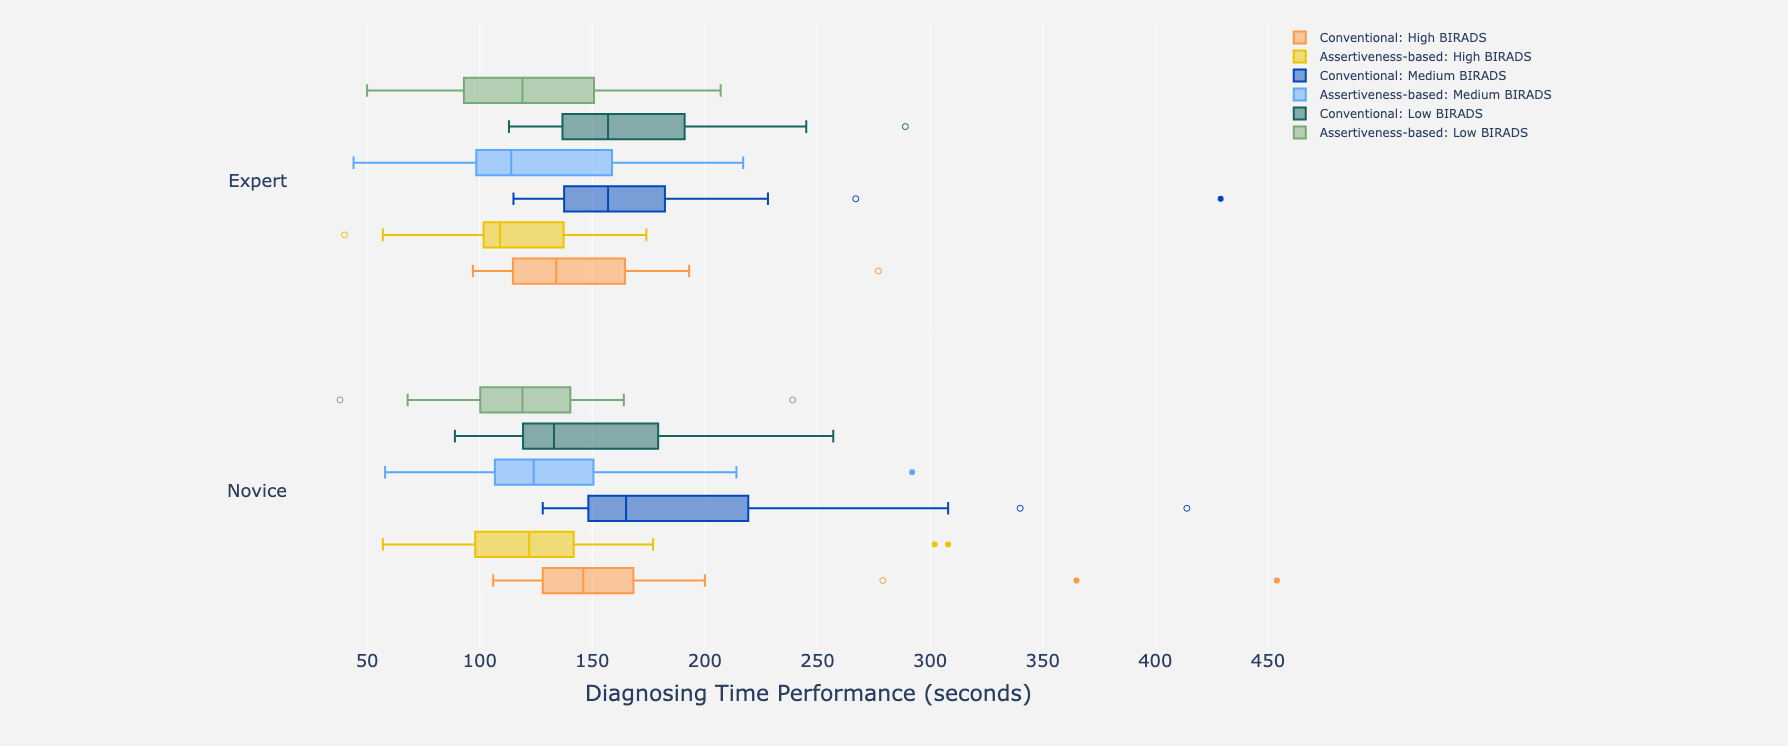
\includegraphics[width=1.000\textwidth]{fig099}
\caption[]{Diagnosing time performance in seconds of novice and expert clinicians to fully diagnose one patient. Different colors are representing different agent trials and breast severities of a patient. Clinicians' task was to read each patient and provide a final BIRADS classification by {\it accepting} or {\it rejecting} the AI recommendations.}
\label{fig:fig099}
\end{figure}
%%%%%%%%%%%%%%%%%%%%%%%%%%%%%%%%%%%%%%%%%%%%%%%%%%%

The impact of an assertiveness-based agent on medical assessments was investigated in this section.
We hypothesized that assertive communication between clinicians and the intelligent agent would alter clinicians' workflow and improve their time performance ({\bf H6.1.1}).
The results confirmed this hypothesis, as the time performance of clinicians improved significantly when using the assertiveness-based agent compared to the conventional agent (Figure~\ref{fig:fig099}).
The difference was statistically significant (F = 11.32, p = 0.005 $<$ 0.05), indicating a large effect size (r = 0.49).

\textcolor{revised}{In testing our hypothesis (\textbf{H6.1.2}), we aimed to determine if the assertiveness-based agent influenced clinicians' diagnostic accuracy.
The results showed no significance (F = 1.85, p = 0.37 $>$ 0.05) in accuracy between the assertiveness-based agent and the conventional agent (Figure~\ref{fig:fig084}).
These findings suggest that the assertiveness level of the agent's explanations does not impact negatively on clinicians' ability to accurately classify patients.
However, it's important to note that a non-significant result does not necessarily imply equivalence in performance between the two conditions.}

%%%%%%%%%%%%%%%%%%%%%%%%%%%%%%%%%%%%%%%%%%%%%%%%%%%
\begin{figure}[htpb]
\centering
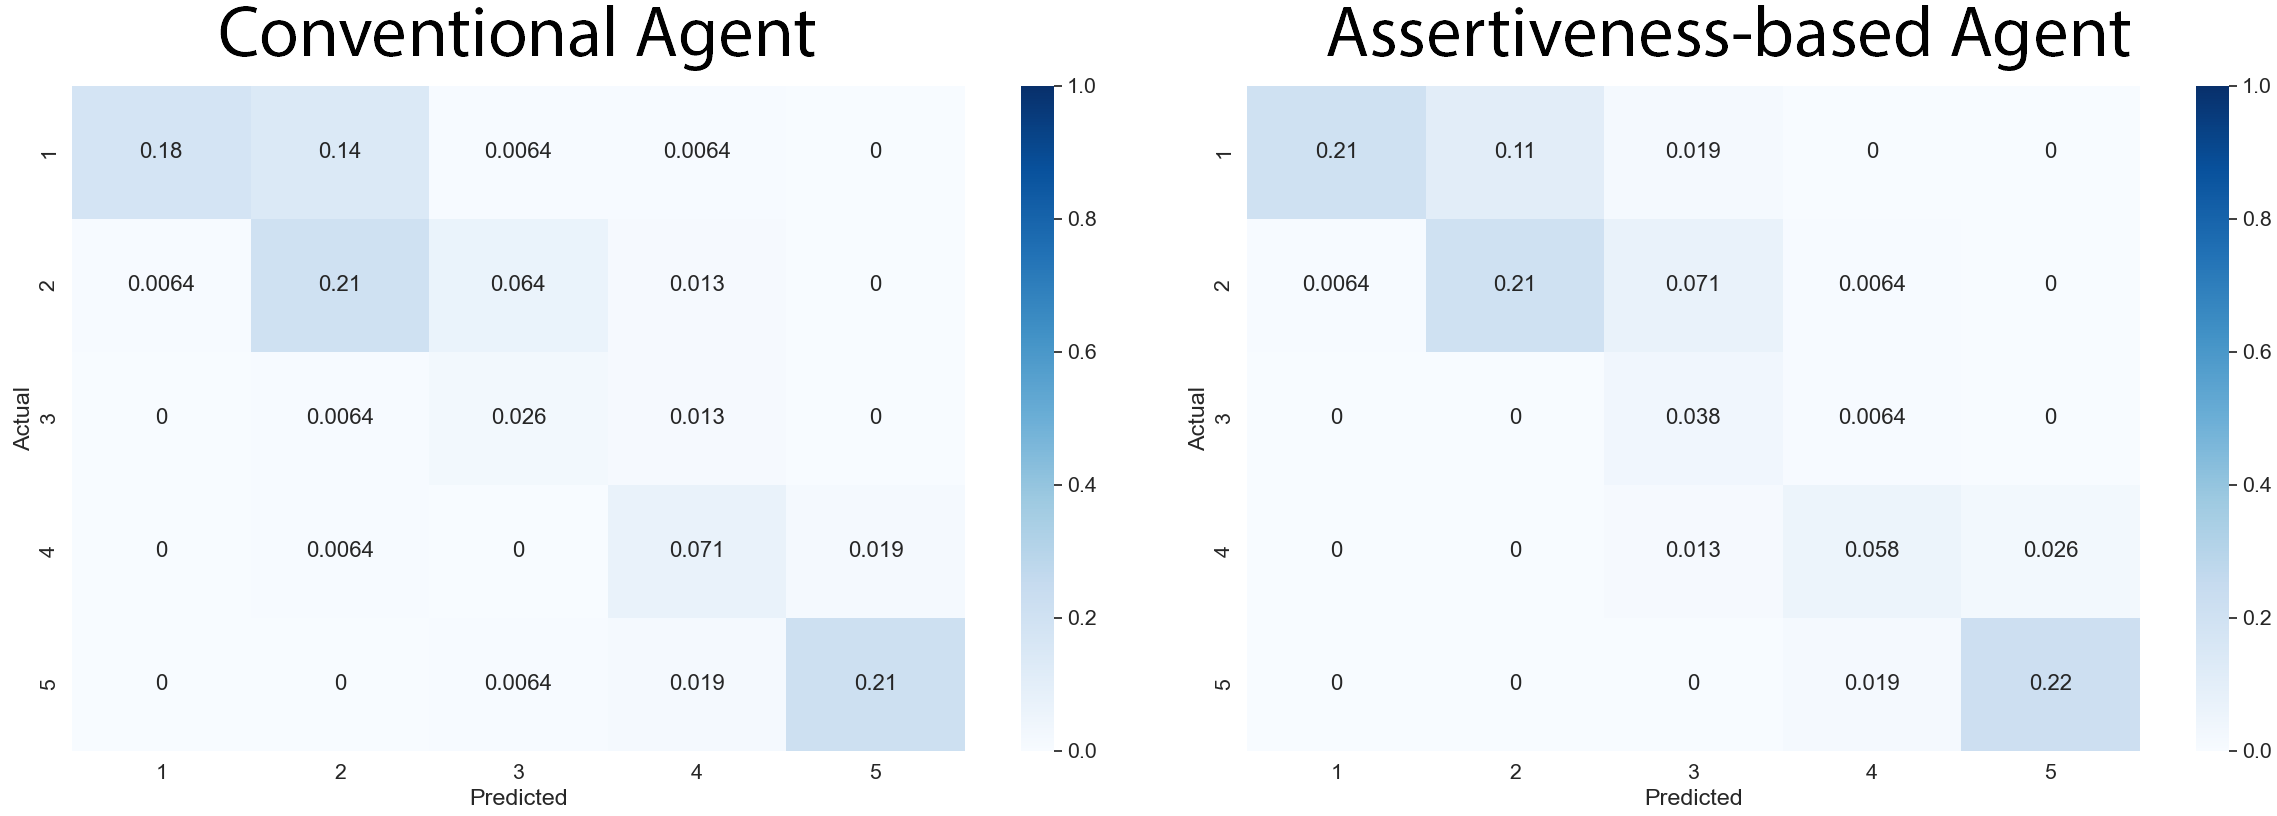
\includegraphics[width=0.855\textwidth]{fig084}
\caption[]{Accuracy rates using a confusion matrix. Comparison between the clinician's BIRADS classification (from 1 to 5) of a patient while using both conventional (left) and assertiveness-based (right) agents. Columns are representing the {\it Predicted} value (collaboration between the clinician and AI), and the rows are representing the {\it Actual} category (biopsy confirmed).}
\label{fig:fig084}
\end{figure}
%%%%%%%%%%%%%%%%%%%%%%%%%%%%%%%%%%%%%%%%%%%%%%%%%%%

\textcolor{revised}{Table~\ref{tab:tab018} provides insights into how clinicians accepted or rejected \ac{AI} recommendations, indicating differences in their responses to assertive versus non-assertive communication styles.
This table shows novice clinicians favor assertive agents, while experts achieve better accuracy with non-assertive agents.
For more detailed results and understanding of these patterns, especially related to clinicians' experience and decision-making effectiveness, see Table~\ref{tab:tab014} in Section~\ref{sec:app005007001} of Appendix~\ref{chap:app005}.}

%%%%%%%%%%%%%%%%%%%%%%%%%%%%%%%%%%%%%%%%%%%%%%%%%%%
\begin{table}[htpb]
\centering
\begin{tabular}{|c|cc|ll|}
\hline
\multirow{2}{*}{\textbf{Trials}} & \multicolumn{2}{c|}{\textbf{Overall Corrects}} & \multicolumn{2}{c|}{\textbf{Overall Mistakes}} \\ \cline{2-5} 
                & \multicolumn{1}{c|}{\textbf{Novice}}         & \multicolumn{1}{c|}{\textbf{Expert}}        & \multicolumn{1}{c|}{\textbf{Novice}}         & \multicolumn{1}{c|}{\textbf{Expert}}        \\ \hline
\textbf{Conventional}        & \multicolumn{1}{c|}{{\color[HTML]{9A0000} 69.70\%}}       & {\color[HTML]{9A0000} 63.77\%}      & \multicolumn{1}{l|}{{\color[HTML]{9A0000} 30.30\%}}       & {\color[HTML]{9A0000} 36.23\%}      \\ \hline
\textbf{Assertive}           & \multicolumn{1}{c|}{{\color[HTML]{009901} 81.59\%}}       & 65.76\%      & \multicolumn{1}{l|}{{\color[HTML]{009901} 18.41\%}}       & 34.25\%      \\ \hline
\textbf{Non-Assertive}       & \multicolumn{1}{c|}{75.63\%}       & {\color[HTML]{009901} 66.41\%}      & \multicolumn{1}{l|}{24.37\%}       & {\color[HTML]{009901} 33.59\%}      \\ \hline
\end{tabular}%
\caption{Percentage of clinicians' acceptance/rejection of \acs{AI} recommendations. Shows how often clinicians switched conclusions after interacting. ``Overall Corrects'' indicates correct acceptance/rejection. ``Overall Mistakes'' denotes incorrect acceptance/rejection.}
\label{tab:tab018}
\end{table}
%%%%%%%%%%%%%%%%%%%%%%%%%%%%%%%%%%%%%%%%%%%%%%%%%%%

Furthermore, we examined the impact of personalized explanations by customizing the agent's communication for novice and expert clinicians (\textbf{H6.1.3}).
The results revealed a significant association ($\chi^2$ = 3.84, p = 0.001 $<$ 0.05) between the agent's communication tone and medical professional experience.
Novice clinicians had a higher chance of correctly classifying a patient with the assertive agent, while expert clinicians had a slightly higher chance with the non-assertive agent.
These findings suggest tailoring the agent's assertiveness to the clinician's experience level.

The analysis also compared switching decision rates between the assertiveness-based and conventional agents.
The results showed that clinicians made better decisions with assertiveness-based assistance, resulting in higher correct acceptance and rejection rates than the conventional condition.
This highlights the importance of scenario design in evaluating clinicians' performance.

\subsection{RQ6.2: Perception of Clinicians towards an Assertiveness-Based Agent}
\label{sec:chap006006002}

\textcolor{revised}{In this section, we provide a summarized overview of our investigation into question {\bf RQ6.2}.
However, for a more comprehensive understanding of our research findings, we present a detailed analysis in Section~\ref{sec:app005007002} of Appendix~\ref{chap:app005}.
Our study provides a comprehensive understanding of how clinicians perceive and interact with \ac{AI} technology in the context of medical assessments.
This investigation focuses on clinicians' preferences and trust in assertiveness-based \ac{AI} communication, and its implications for \ac{AI} system design in healthcare.
The detailed results in Section~\ref{sec:app005007002} of Appendix~\ref{chap:app005} explore these interactions, providing insights for better tailoring \ac{AI} tools to medical professionals' needs.}

\textcolor{revised}{Clinician feedback provided insights into their experiences and attitudes towards the assertiveness-based and conventional agents.
Our statistical analysis revealed a significant preference (F = 8.35, p = 0.001 $<$ 0.05) for the assertiveness-based agent, with 66\% of participants indicating a favor towards it (Figure~\ref{fig:fig085}), as hypothesized in {\bf H6.2.1}.
Conversely, 24\% of the clinicians showed a preference for the conventional agent, and the remaining 10\% did not express a specific choice.
These results highlight clinician receptiveness to assertiveness-based in \ac{AI} communication, suggesting its usefulness in medical decision-making.
Therefore, clinicians' preference for the assertiveness-based agent underscores the need for flexible, personalized \ac{AI} communication strategies.}

%%%%%%%%%%%%%%%%%%%%%%%%%%%%%%%%%%%%%%%%%%%%%%%%%%%
\begin{figure}[htpb]
\centering
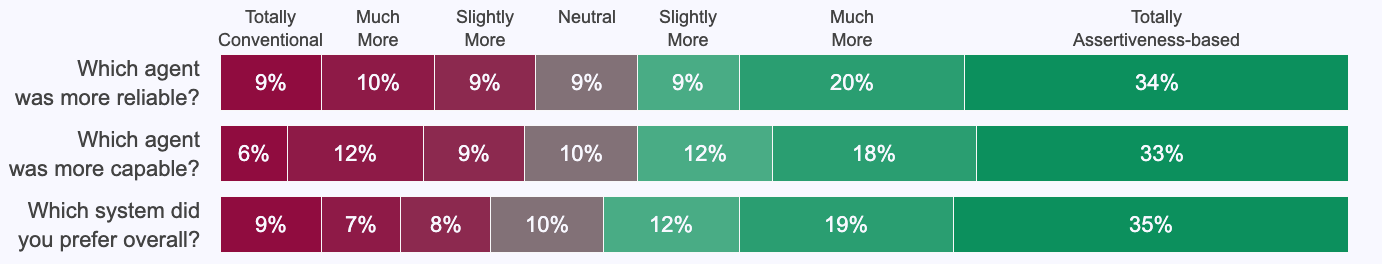
\includegraphics[width=1.000\textwidth]{fig085}
\caption[]{Preference choices of clinicians when comparing both conventional and assertiveness-based agents within this study. Rates of clinicians are ranging from {\it Totally Conventional} to {\it Totally Assertiveness-based} on perceived {\it reliability}, {\it capability}, and {\it overall preference} of each agent.}
\label{fig:fig085}
\end{figure}
%%%%%%%%%%%%%%%%%%%%%%%%%%%%%%%%%%%%%%%%%%%%%%%%%%%

\textcolor{revised}{In our study, we assessed clinicians' perceptions of trust, understanding, competence, and thoughtfulness towards both conventional and assertiveness-based agents, as detailed in Table~\ref{tab:tab013}.
The statistical analysis revealed no significant difference in perceived trustworthiness between the two agents (F = 19.47, p = 0.06 $>$ 0.05).
Similarly, understanding levels did not show significant differences (p = 0.14 $>$ 0.05).
However, the assertiveness-based agent was rated significantly higher in terms of perceived competence (p = 0.04 $<$ 0.05) and elicited higher thoughtfulness from clinicians (p = 0.001 $<$ 0.05).
These findings imply a nuanced response to \ac{AI} agents' communication styles, but interpretation requires caution.
Non-significant differences in trust and understanding don't imply equivalence.
These results partially support our hypothesis ({\bf H6.2.2.}) on clinicians' preferences, underscoring the value of personalized \ac{AI} communication in healthcare.}

%%%%%%%%%%%%%%%%%%%%%%%%%%%%%%%%%%%%%%%%%%%%%%%%%%%
\begin{table}[htpb]
\resizebox{\textwidth}{!}{%
\begin{tabular}{ccc}
\hline
Questions                                                            & Conventional & Assertiveness-based \\ \hline
Overrall, I can trust in the agent recommendations.                  & 86\%         & 90\%                \\
I understand what the system is thinking.                            & 91\%         & 94\%                \\
The system seems competent.                                          & 82\%         & 92\%                \\
The agent shows great thoughtfulness while dealing with the patient. & 71\%         & 75\%                \\ \hline
\end{tabular}%
}
\caption[]{Comparison for the percentage of agreement between conventional and assertiveness-based agents. The questions are following the three {\it dimensions of trust} represented by perceived {\it understanding}; {\it competence}; and {\it thoughtfulness}.}
\label{tab:tab013}
\end{table}
%%%%%%%%%%%%%%%%%%%%%%%%%%%%%%%%%%%%%%%%%%%%%%%%%%%

\textcolor{revised}{We analyzed workload and usability between conventional and assertiveness-based agents using both \ac{NASA-TLX} and \ac{SUS} measurements.
Results indicated no significant workload or usability differences between the two agent conditions (p = 0.38 $>$ 0.05).
Therefore, these findings support our hypothesis ({\bf H6.2.3.}) that assertiveness-based communication in \ac{AI} agents wouldn't affect clinicians' workload or usability.
This suggests that assertiveness-based in \ac{AI} communication can be integrated without compromising the ease of use or increasing the cognitive burden on clinicians.}

Last, we examined how clinicians perceive the levels of assertiveness in communicating clinical arguments (Figure~\ref{fig:fig091}).
The results revealed significant differences in reliability (F = 31.36, p = 0.0001 $<$ 0.05) and capability (F = 18.17, p = 0.0003 $<$ 0.05) between novice and expert clinicians.
These findings support our hypothesis ({\bf H6.2.4.}) that clinicians' preferences vary based on the assertiveness level of the agent, indicating differing perceptions of clinical arguments.

%%%%%%%%%%%%%%%%%%%%%%%%%%%%%%%%%%%%%%%%%%%%%%%%%%%
\begin{figure}[htpb]
\centering
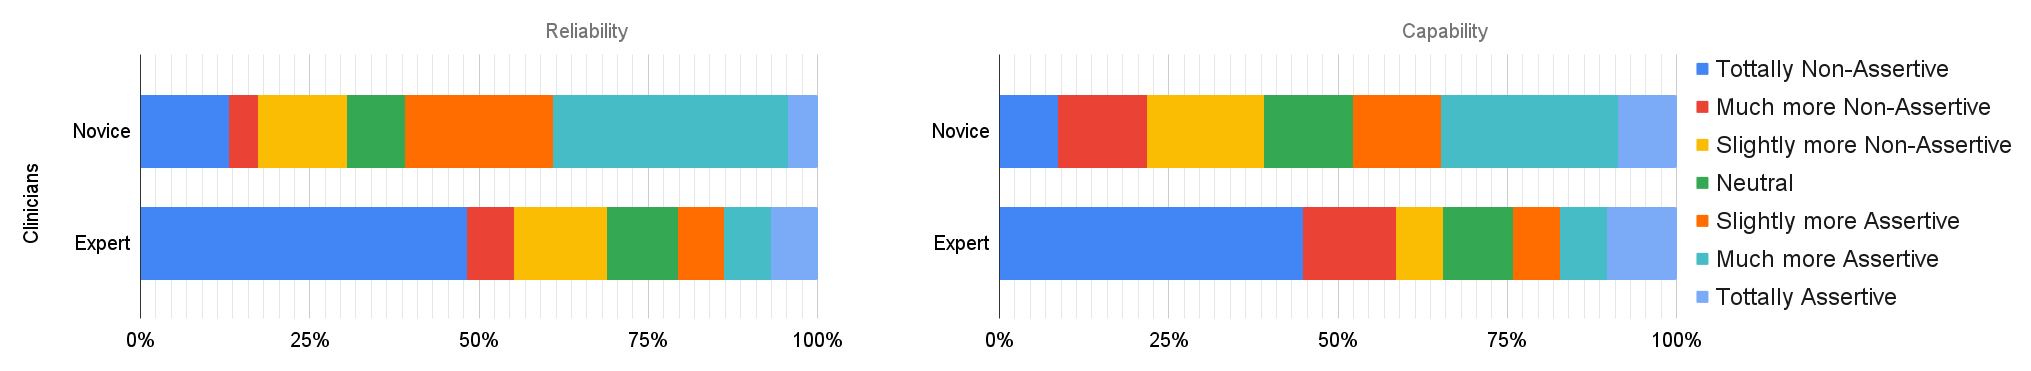
\includegraphics[width=1.000\textwidth]{fig091}
\caption[]{Ratings between novice and expert clinicians for perceived reliability and capability. Clinicians rated each agent, ranging from {\it Totally Non-Assertive} to {\it Totally Assertive} communication.}
\label{fig:fig091}
\end{figure}
%%%%%%%%%%%%%%%%%%%%%%%%%%%%%%%%%%%%%%%%%%%%%%%%%%%

\subsection{Summarized Qualitative Insights}
\label{sec:chap006006003}

\textcolor{revised}{This section presents a synthesis of the qualitative analysis of clinicians' perceptions and experiences with conventional and assertiveness-based agents, further detailed in Section~\ref{sec:app005007003} of Appendix~\ref{chap:app005}.
Our participatory approach analyzed data from 12 focus group sessions over four months (Section~\ref{sec:app005006} of Chapter~\ref{chap:app005}), involving 18 participants with diverse expertise.
In every session, lasting around 40 minutes and comprising about 4 to 8 participants ({\it e.g.}, between clinicians and researchers), we facilitated focused discussions on the usability, interpretability, and efficiency of intelligent agents in clinical decision-making.
We transformed these complex discussions into clear, thematic insights through emergent affinity diagramming, focusing on clinical arguments and the visualization of \ac{AI} recommendations.}

\textcolor{revised}{Our analysis, detailed in Section~\ref{sec:app005007003001} of Appendix~\ref{chap:app005}, showed a clear clinician preference for human-interpretable arguments over numerical \ac{AI} outputs, with 92\% favoring the assertiveness-based agent's personalized communication.
This preference was linked to the agent's precise, meaningful explanations of \ac{AI} recommendations.
A junior clinician noted: ``{\it The assertiveness-based gave me a better understanding of the \acs{AI}'s reasoning, which helped me make more informed decisions}'' (C6).
Our findings, as elaborated in Section~\ref{sec:app005007003002} of Appendix~\ref{chap:app005}, also revealed how clinicians' mental models of intelligent agents are shaped by their experiences and expectations.
One clinician remarked: ``{\it The first \acs{AI} [assertiveness-based] was outstanding... but in the second \acs{AI} [conventional] I was frustrated with the lack of communication in comparison to the first one}'' (C48).
Expert clinicians used communication tone to gauge \ac{AI} recommendation reliability, while novices focused on learning and patient comparisons.}

\textcolor{revised}{These findings underscore the necessity for personalized and adaptable communication in \ac{AI} systems, catering to clinicians' diverse needs and expertise levels.
They align with the discussions in Section~\ref{sec:chap005007003} of Chapter~\ref{chap:chap005}, reinforcing the importance of user-centered design in the development of \ac{AI} systems for clinical decision-making~\cite{10.1145/3491102.3517789}.
Our research contributes to the broader understanding of how \ac{AI} communication styles influence clinician decision-making, highlighting the need for \ac{AI} systems that are technically proficient and attuned to user needs and preferences.}

\section{Discussion}
\label{sec:chap006007}

In this section, we provide a condensed overview of the in-depth discussion presented in Section~\ref{sec:app005008} of Appendix~\ref{chap:app005}, where we explore the insights derived from our study and offer targeted recommendations for designing and integrating intelligent agents into the field of medical imaging.
We studied how personalized and customized communication of an intelligent agent can aid clinicians in their decision-making during medical imaging diagnosis.
We conducted a within-subject to investigate how clinicians perceive assertiveness-based agents differently.
Our results show that assertiveness-based agents can alter clinicians' workflows by increasing the efficiency of clinicians while maintaining overall efficacy.

Our findings revealed that the classification accuracy was unaffected by assertiveness-based communication.
However, the tone of the explanations had a significant influence on the decision-making behavior of novice and expert clinicians.
This emphasizes the need for compliant agents that provide personalized and tailored explanations.
By addressing this, future developments can focus on enhancing the provision of relevant and customized explanations, ultimately improving the effectiveness of intelligent agents in medical imaging diagnosis.
These insights contribute to healthcare, \ac{HCI}, decision support, and \ac{AI} communication research.

\subsection{Design Implications}
\label{sec:chap006007001}

This section explores valuable design implications for developing innovative \ac{AI} systems in the clinical domain.
It covers various topics such as combining diverse knowledge classifiers (Section~\ref{sec:app005008001001}), enriching training methods with additional information (Section~\ref{sec:app005008001002}), and designing intuitive and user-friendly \acp{UI} for effective agent communication (Section~\ref{sec:app005008001003}).
The generalizability and broader applicability of the study to other related fields are also discussed (Section~\ref{sec:app005008001004}).
Further in-depth insights and recommendations can be found in Section~\ref{sec:app005008001} of Appendix~\ref{chap:app005}.

\textcolor{revised}{In breast cancer diagnosis, integrating comprehensive patient information into \ac{AI} systems aligns with clinicians' mental models, essential for enhancing decision-making (Section~\ref{sec:app005008001001}).
\ac{DL} methods must interpret clinical data and customize communication to match clinicians' experiences and backgrounds, adapting to various data types in clinical workflows.
This customization can be achieved through integrated training or distinct \ac{DL} methods for each data type.
Tailored communication, enriched with patient-specific details, improves outcomes in medical imaging.
Modulating communication tone enhances the \ac{AI} system's effectiveness and trustworthiness.}

\textcolor{revised}{Our study emphasizes personalized agent communication in medical imaging, extending beyond the integration of granular patient data from mixed \ac{DL} classifiers.
This approach involves dynamically adapting communication tone to align with clinicians' medical experience, requiring \ac{DL} methods to predict mixed clinical parameters on the far side of traditional diagnostic criteria (Section~\ref{sec:app005008001002}).
Customizing communication tone should cater to clinicians' diverse demographics, achievable through unified training or distinct \ac{DL} methods for specific clinical variables.}

\textcolor{revised}{Evaluating personalized communication between agents and clinicians with varying expertise is achieved by adapting communication tone (Section~\ref{sec:app005008001003}).
Initial findings indicate a need for more research into clinicians' demographics and agent behaviors, such as proactive and reactive behaviors.
Qualitative data show clinician preference for communication styles matching the \ac{AI}'s belief level, emphasizing the need for tone adaptability in \ac{AI} recommendations (Section~\ref{sec:app005015}).
An intelligent agent might be {\it assertive and proactive} when the \ac{DL} method is highly competent or, otherwise, more {\it suggestive and reactive}, aligning communication with clinical context-awareness and decision-making characteristics.}

\textcolor{revised}{Future research should prioritize the exploration of intelligent agents that tackle the generalizability of \ac{DL} methods (Section~\ref{sec:app005008001004}), incorporating diverse data to enhance clinical workflow integration~\cite{RASMY201811}.
These agents, especially those using assertiveness-based communication, must adapt their tone to the belief level of their explanations, improving medical \ac{AI} systems and fostering human-centered design.
In clinical scenarios with data variability, the communication tone should reflect the \ac{DL} model's generalizability, being suggestive for limited data and assertive for well-represented cases.
Caution is necessary when applying this study's findings to other medical areas, but the identified personalized communication methods may benefit various diagnoses due to common challenges across specialties.}

\subsection{Limitations}
\label{sec:chap006007002}

This section summarizes the analysis of the study constraints discussed in Section~\ref{sec:app005008002} of Appendix~\ref{chap:app005}.
The study on assertiveness-based agents in breast cancer diagnosis faced challenges due to limited clinician availability and remote study conditions, impacting task control and clinician interactions.
Liability implications in medical settings and evolving legal frameworks present further limitations, requiring research and legal developments.
Future efforts should focus on robust frameworks and guidelines to address risks and establish accountability.
Training personalized \ac{DL} models and exploring different agent features are areas for future exploration.

\section{Conclusion}
\label{sec:chap006008}

In this work, we provide a novel perspective on how to personalize and customize the explanations of intelligent agents to human clinicians.
Our results from an experimental study with 52 clinicians comparing a conventional agent to an assertiveness-based agent suggest that the ability of a system to not only exploring how to adapt the communication tone ({\it i.e.}, more suggestive or more assertive), but also provide granular explanations of patient cases has merits for end users.
From our results, the time performance was satisfactory, where clinicians took less 25\% of the time to diagnose a patient with the assertiveness-based agent in comparison to the conventional agent.
As we observed, the comparison between the conventional agent and the assertiveness-based agent was also more effective with the latter in achieving the proper diagnostic of the patient.
Additionally, our results demonstrate that if explanations are adapted taking into account the medical experience of clinicians, accuracy chance of correctly diagnosing a patient is 91\% higher for novice and 78\% higher for expert clinicians.
Last, clinicians are showing an increase in trust, preferring the assertiveness-based agent by being more reliable and capable, as this agent was revealing to be further understandable, competent and thoughtful.
Our work has implications for the design of \ac{AI} systems not only in the medical domains, but also in fields that are facing similar challenges, demanding a personalization of the human-AI interaction.